\section{Linguistic tools}

One of the main parts of Reprotool project is an automatic text analysis. This part allows user to skip long-lasting manual annotation by pushing a button. This chapter describes implementation of linguistics analysis in Reprotool project and its linguistics background.

\subsection{Introduction}
Process of linguistics analysis gets natural language sentences as an input and returns analyzed usecases as is shown at figure \ref{fig:LinguisticsAnalyseSmall}. Whole process is divided into two parts: process of parsing and core analysis. Parsing contains main linguistics operations which are tokenization, tagging, parsing and lemmatization. Core work of parsing process is done by popular external linguistic analysis tools described in section \ref{sec:externaltools}. Core analysis converts parsed sentence trees with annotations into our usecases model. This process is described in more detail in section \ref{sec:analysis}. % TODO \ref{sec:usecasemodel}

Each implementation of any analyse brings problem of measuring success. We have put together a dataset of nearly tree hundred of sentences. These sentences contain the most common use cases operations. All these sentences were manually annotated and analyzed. In section \ref{sec:benchmark} is described our benchmark solution with actual results.

\begin{figure}[ht]
  \centering
  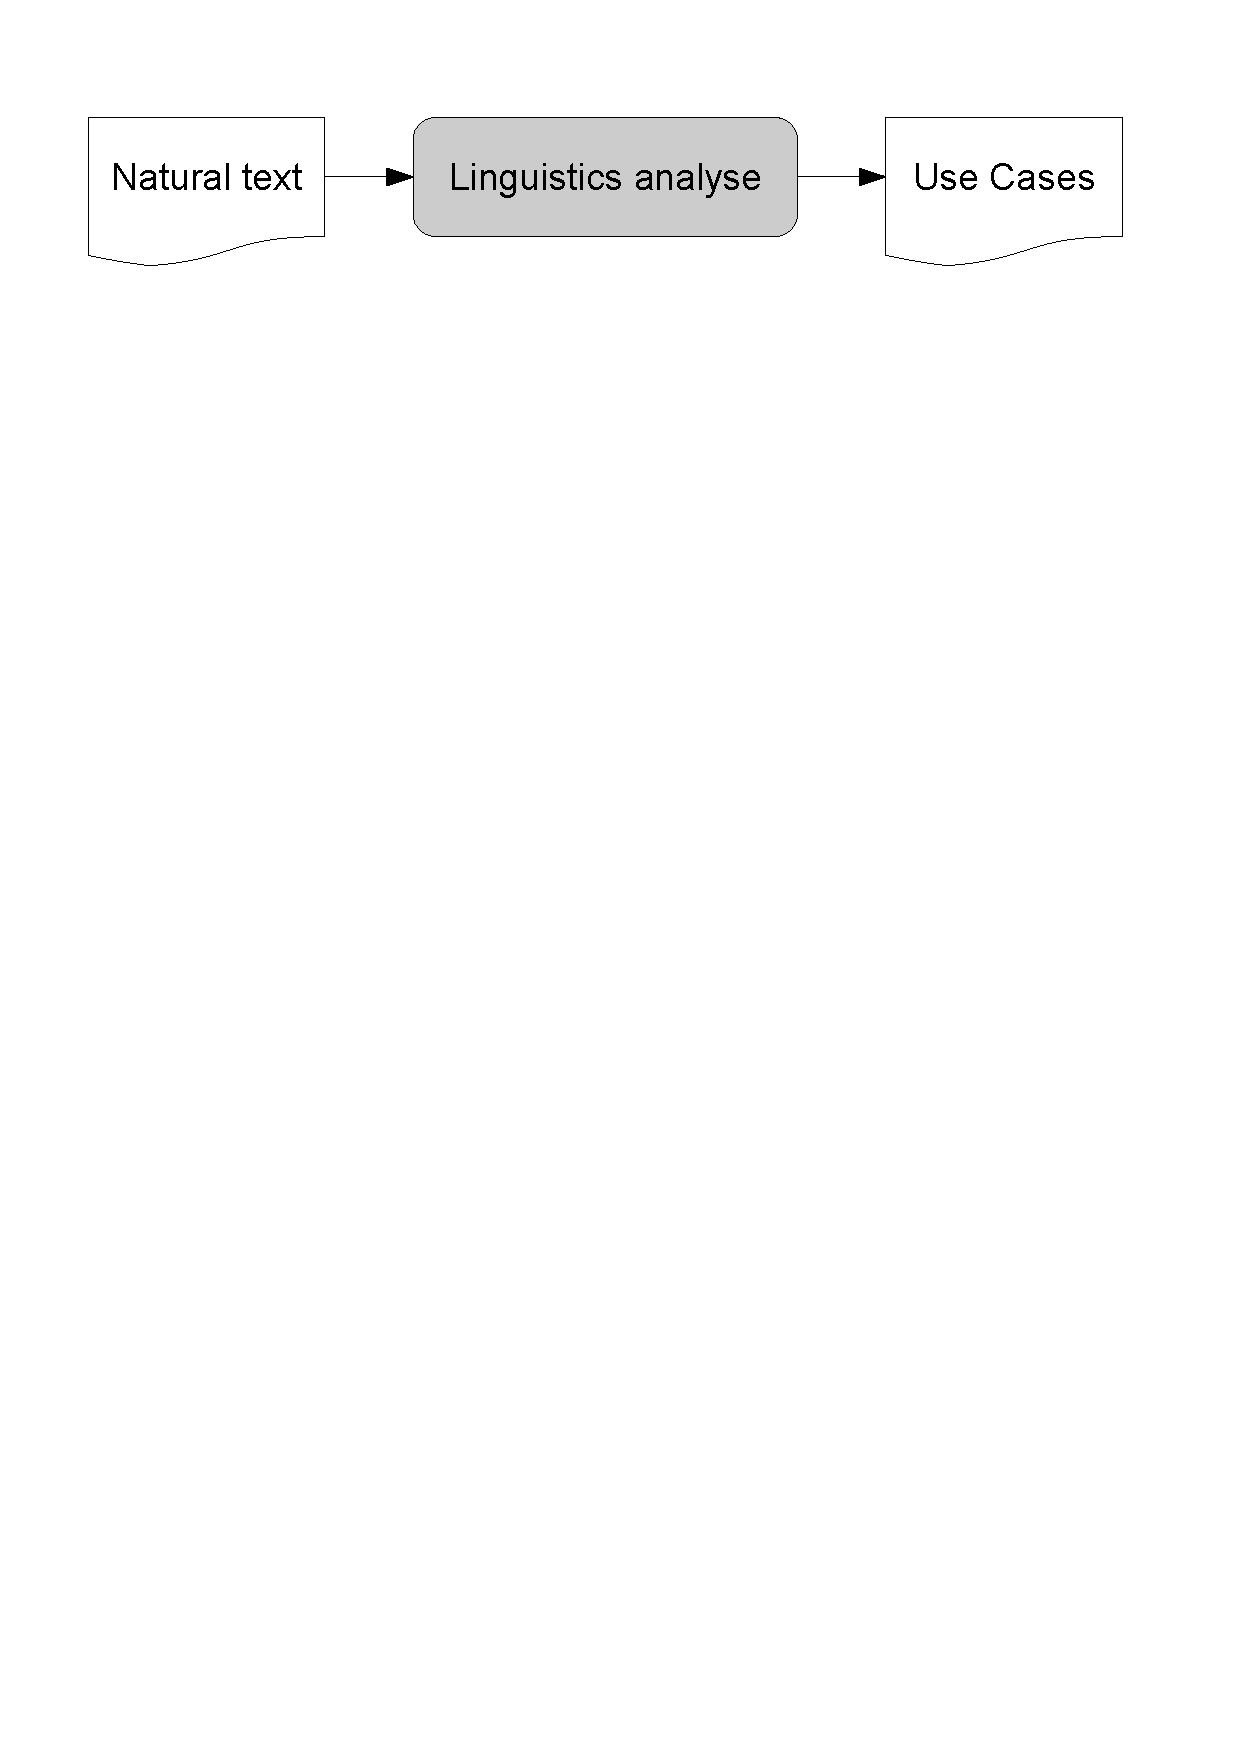
\includegraphics[height=30pt]{images/LinguisticsAnalyseSmall}
  \caption{Process of sentence analysis}
  \label{fig:LinguisticsAnalyseSmall}
\end{figure}

\subsection{External tools}
\label{sec:externaltools}
As described in previous sections, whole linguistics analysis is a hard task to do. Implementing all acts of this work is out of the scope of the project.  Especially parsers do a very sophisticated and difficult tasks. We choose selected commonly used external tools to do some parts of analysis. 

These parts were part-of-speech tagging, sentence parsing and obtaining lemma forms for words. Main reasons for our selection were widespread  and credibility of the tools, at least partial compatibility of output and input formats and Java implementation. 

We demanded Java implementation, because runtime control of programs written in different languages is inoperative and bring big problems in portability of project. The selected tools don't allow access like common internal java classes, but we are able to control their correct running.

Selected tools are:
 
\begin{itemize}
\item {\bf MXPOST tagger} - \href{http://www.inf.ed.ac.uk/resources/nlp/local_doc/MXPOST.html}{Java implementation of well known Maximum Entropy Part-Of-Speech Tagger}
\item {\bf Dan Bikel's Multilingual Statistical Parsing Engine } - Java implementation coming from \href{http://www.cis.upenn.edu/~dbikel/software.html#stat-parser}{Dan Bikel’s Home Page}
\item {\bf Mate-tools lemmatizer} - part of bigger project called \href{http://code.google.com/p/mate-tools/}{Tools for Natural Language Analysis}
\end{itemize}

Larger list of tools could be found at project site. There are also links to similar pages concerned with the same theme. 
          
\subsubsection{MXPOST tagger} 
MXPOST tagger was written in Java implementation at University of Edinburg by NLP group and is maintained as part of theirs NLP tools.
        
Main part of this tagger is based on original parser written by Adwait Ratnaparkhi. Detailed description of this original parser is described in article \cite{Linguistics-ratnaparkhi96} and in his PhD thesis \cite{Linguistics-ratnaparkhi98}. 

This 
Work of 

Input data, natural language sentences, 
Main model of MXPOST tagger relies on the assumption that input sentences are tokenized
according to the Penn Treebank conventions.
  
\subsubsection{Dan Bikel's Multilingual Statistical Parsing Engine}   

\subsubsection{Mate-tools lemmatizer}          
          
\subsection{Analysis}
\label{sec:analysis}

\begin{figure}[ht]
  \centering
  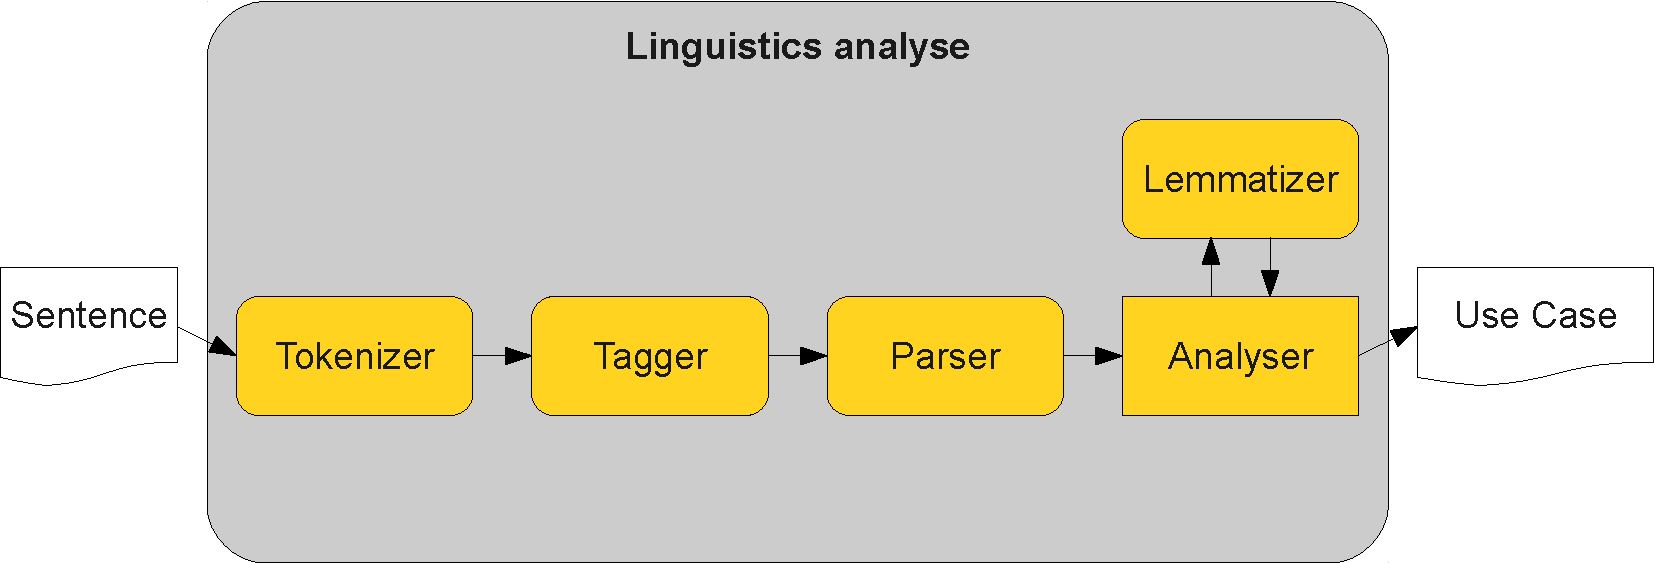
\includegraphics[width=300pt]{images/LinguisticsAnalyse}
  \caption{Process of sentence analysis}
  \label{fig:LinguisticsAnalyse}
\end{figure}

\subsubsection{Tokenization}
\begin{table}[ht]   % or b
\begin{center}
    \begin{verbatim}
Input 	Natural language sentence; negation detection
Output 	Array of tokens (eg. words, numbers) 
        \end{verbatim}
  \caption{Tokenizer data}
  \label{tab.tokenization}
\end{center}
\end{table} 

\subsubsection{Tagging}
\begin{table}[ht]   % or b
\begin{center}
    \begin{verbatim}
Input 	Array of tokens
Output 	Array of POS tagged tokens (eg. adjectives, verbs) 
        \end{verbatim}
  \caption{Tagger data}
  \label{tab.tagging}
\end{center}
\end{table} 

\subsubsection{Parsing}

\begin{table}[ht]   % or b
\begin{center}
    \begin{verbatim}
Input 	Array of POS tagged tokens
Output 	Parse trees of each sentence 
        \end{verbatim}
  \caption{Parser}
  \label{tab.parsing}
\end{center}
\end{table}  

\subsubsection{Lemmatization}
\begin{table}[ht]   % or b
\begin{center}
    \begin{verbatim}
Input 	Parse trees of each sentence
Output 	Lemma for each word 
        \end{verbatim}
  \caption{Example output from benchmark plug-in}
  \label{tab.parsing}
\end{center}
\end{table} 

\begin{figure}[ht]
  \centering
  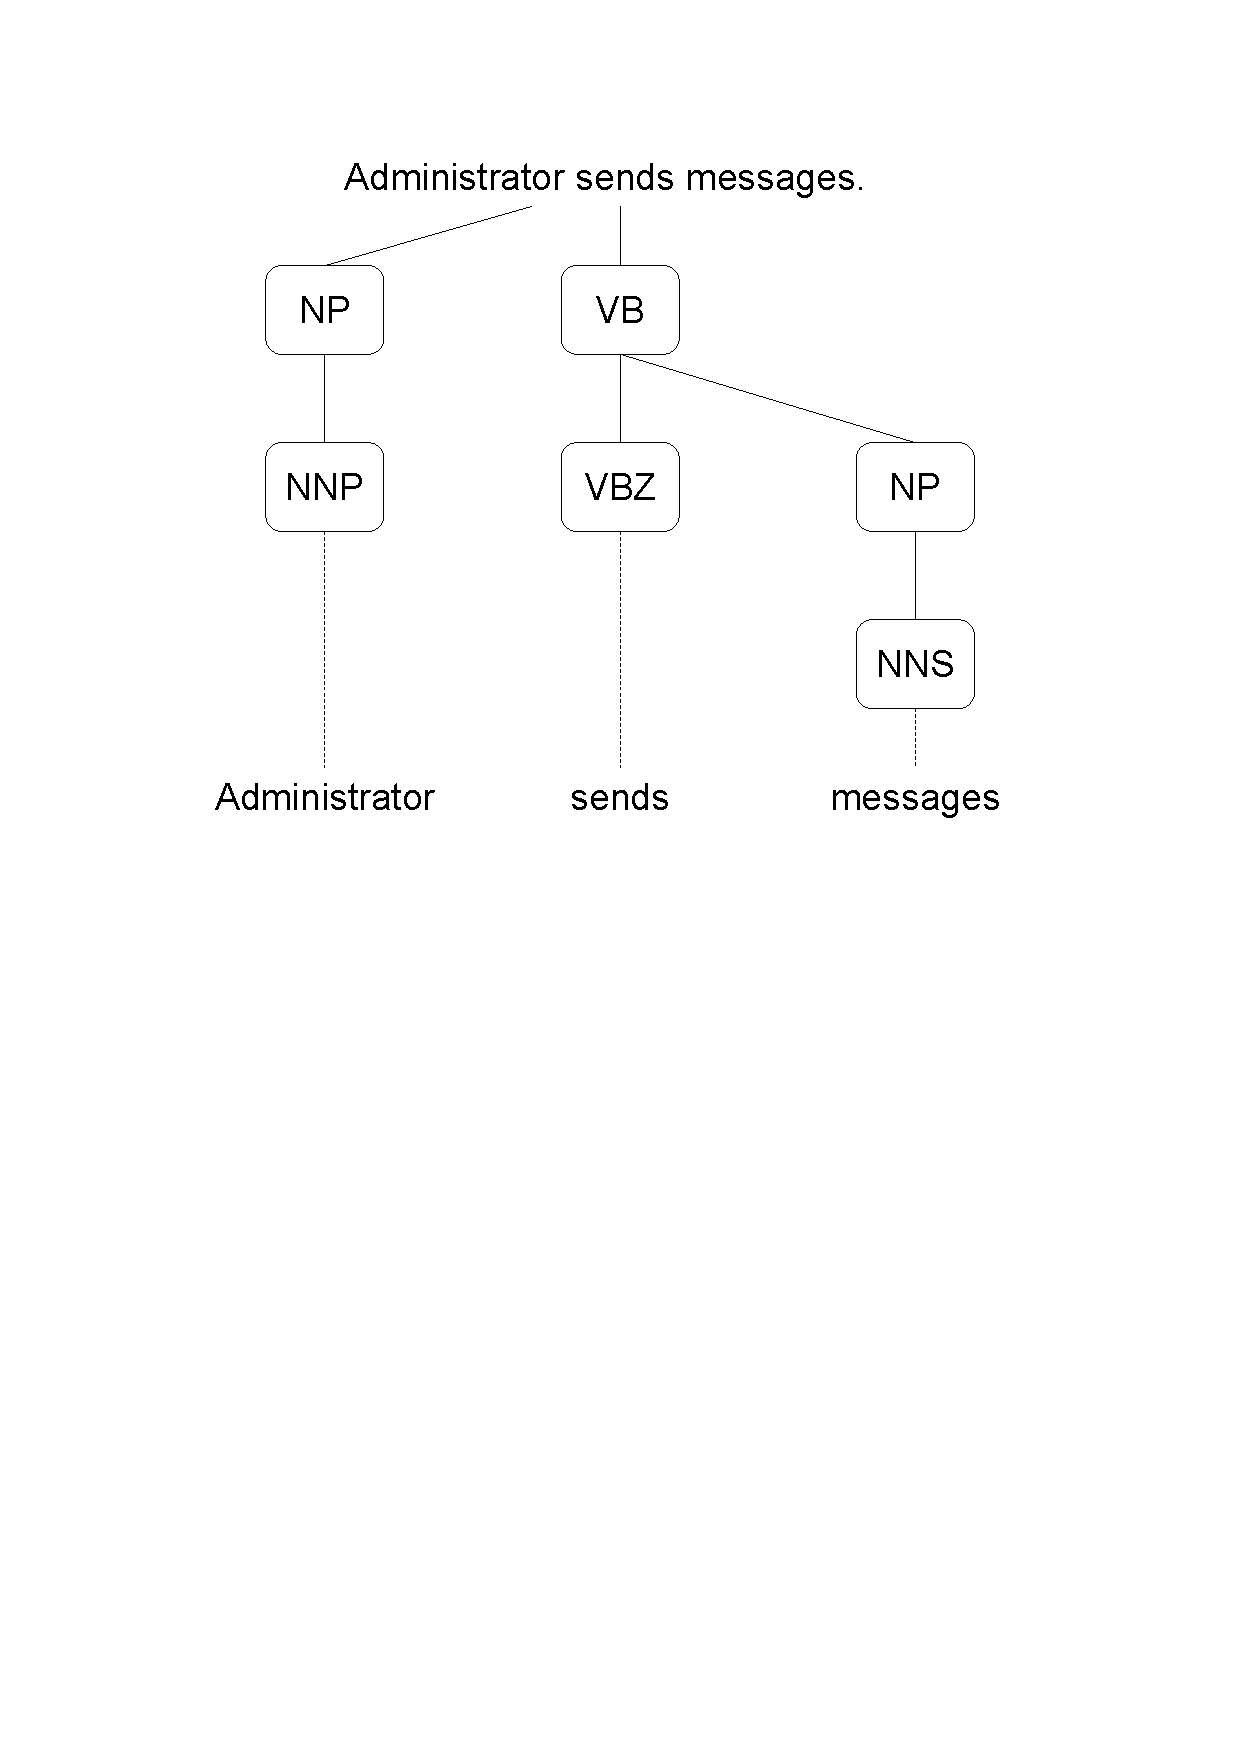
\includegraphics[width=200pt]{images/ParsedTree}
  \caption{Parsed tree of sentence "Administrator sends messages".}
  \label{fig:ParsedTree}
\end{figure}

\begin{figure}[ht]
  \centering
  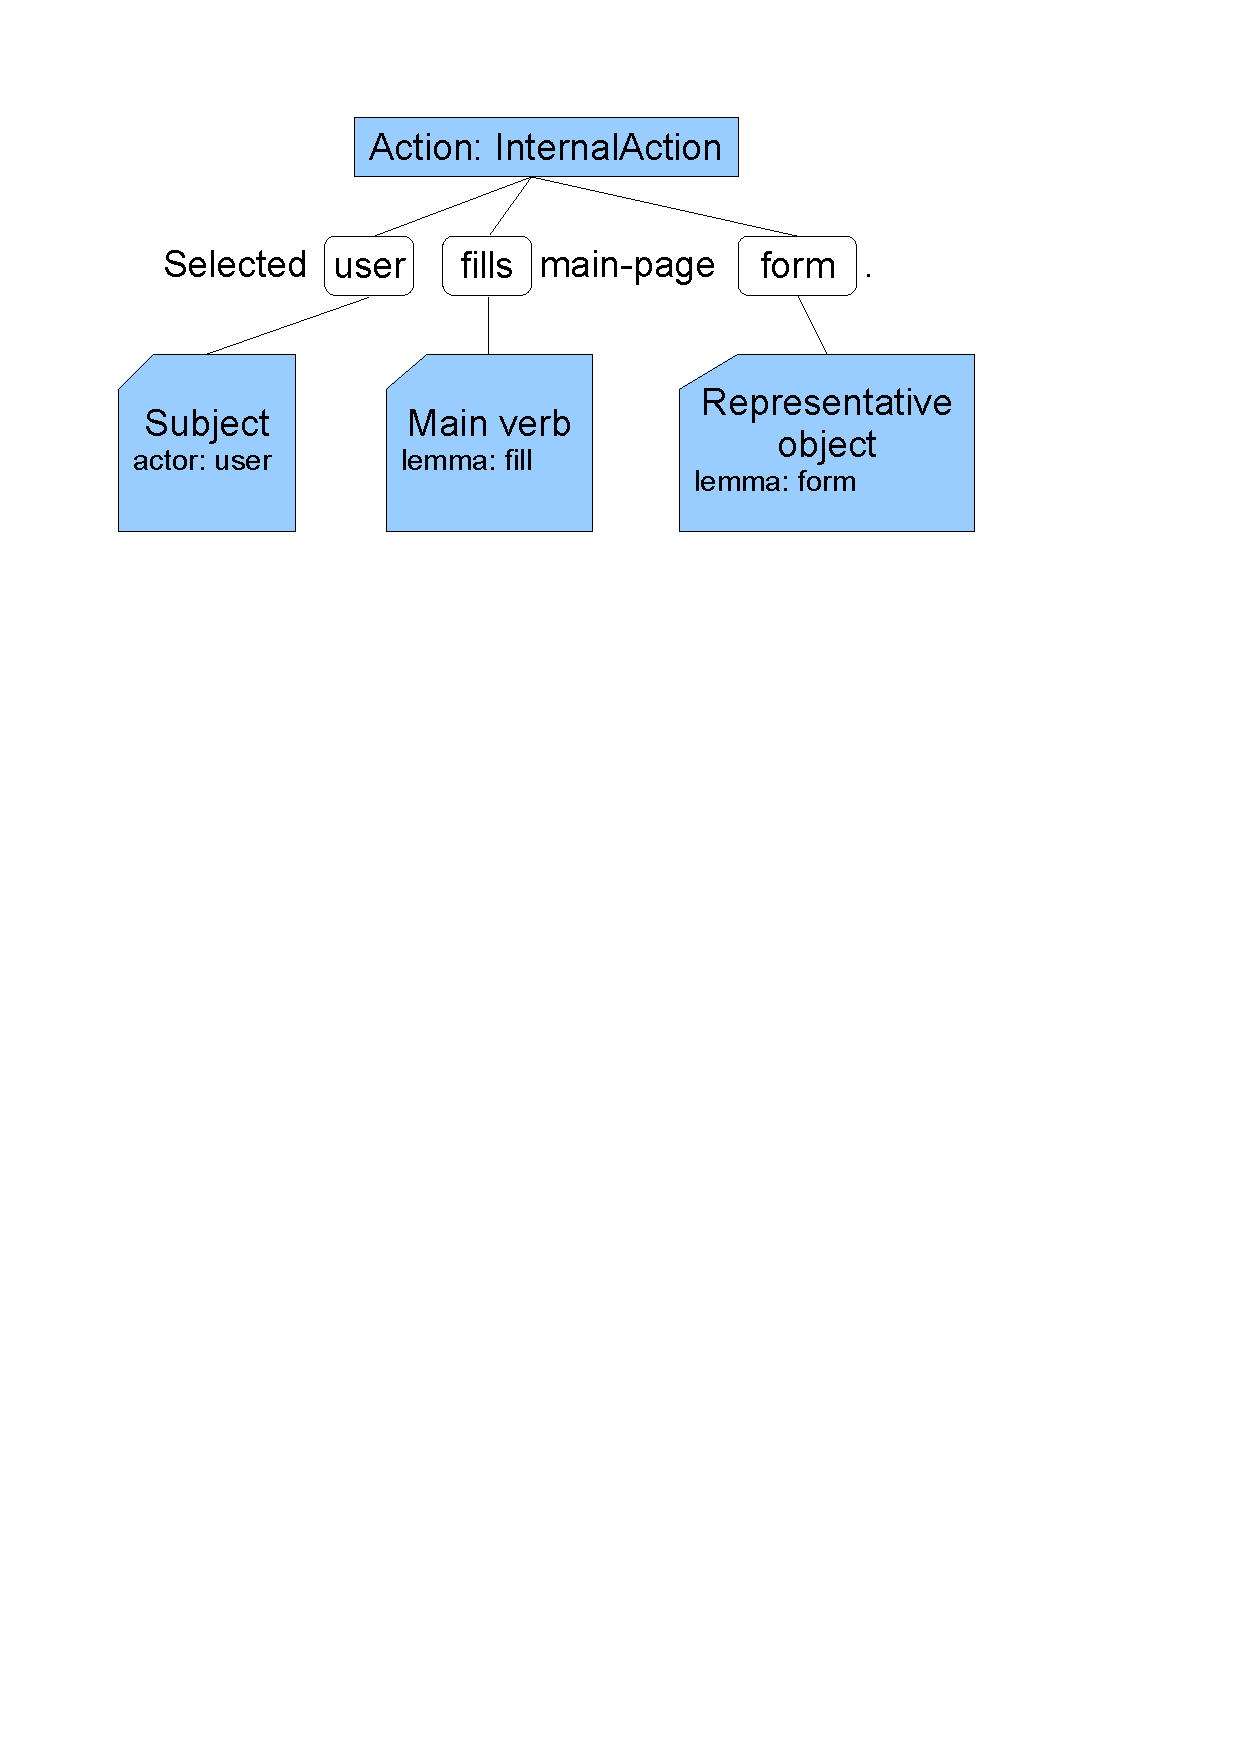
\includegraphics[width=250pt]{images/InternalActionExample}
  \caption{Example of internal action analysis result.}
  \label{fig:InternalActionExample}
\end{figure}

\begin{figure}[ht]
  \centering
  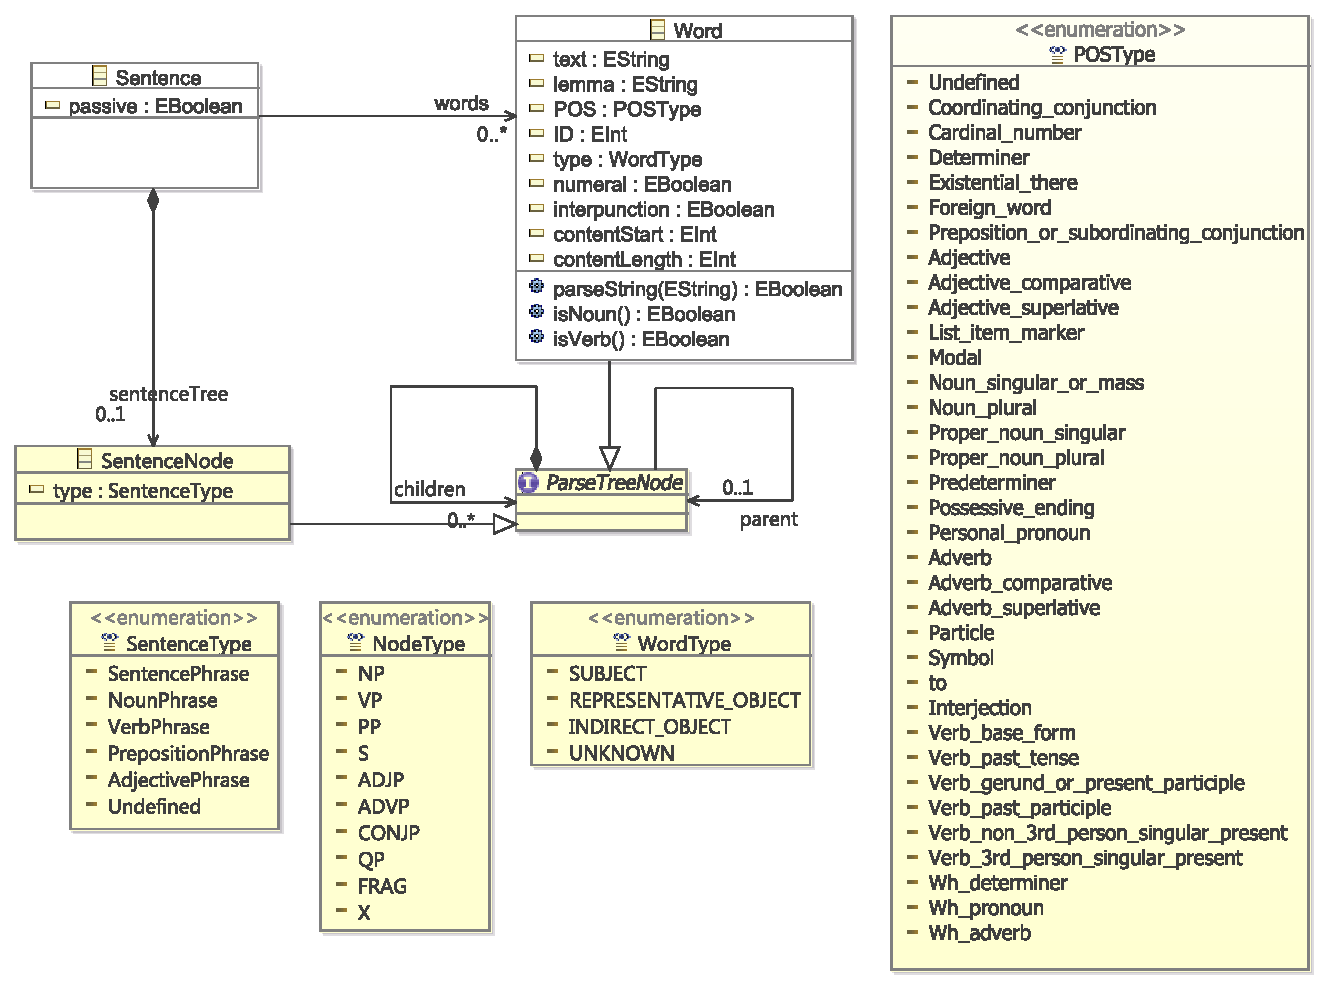
\includegraphics[width=\textwidth]{images/ReprotoolLingModel}
  \caption{Internal linguistics model with enumerations.}
  \label{fig:ReprotoolLingModel}
\end{figure}

\subsection{Linguistics background}

Main goal of linguistic analyse in our porject is to identify important words in a sentence. These words are mainly constituents. For our purpose, we are identifiing four groups of words:

\begin{itemize}
\item {\bf Subject} main subject of the sentence
\item {\bf Main verb} verb wearing meaning
\item {\bf Representative object} main subject of sentence action
\item {\bf Indirect object} an actor usually owning representative object
\end{itemize}

These words are used in action analysis. We are matching sentences to proper actions with a set o deriving rules, which are based on these words. 
                                                                    
\subsubsection{Subject}
For our purpose, subject must be always an actor. User have to add sentence actors before analysis. Usually is subject noun in a top noun phrase. If the sentence is in passive, subject stands at object's place. 

Subject could be also missing. In that case analysis still tries to find other constituents.

There are two predefined actors, "system" and "user". These actors could be subjects without user interaction.

\subsubsection{Main verb}
This verb is a main verb of highest verb phase in a sentence. In a passive sentence is auxiliary verb ingnored. 

Finding verb is in properly parsed sentence easy task, but in a sentence with a wrong parsed tree usually culodn be found. It happens usually when parsed don't know current verb.

\subsubsection{Indirect object}
We are deriving first indirect objects and after then representative (conceptual) objects. All indirect object are actors and indirect objects aren't in the same node with other objects.

Node with indirect objects must be noun phrase which is in verb phrase. If this node is found, all objects are marked as indirect. Indirect object cannot be in possessive form.  


\subsubsection{Representative object}
Representative object could be noun in a noun phrase which is a child of main verb phrase. Except noun phrase with indirect objects.

If a phrase contains more nouns without conjunction, we mark as an object last of the nouns.

\subsection{Actions deriving rules}
When we have all constituents, analysis cant continue with determining proper action and filling internal models with obtained data from analysis.

Types of actions come from our usecase model, which is restricted due to exporting purpose. Overall small action set allows various export options described in previous chapters.

\subsubsection{Include usecase action}


\subsubsection{Goto action}

\subsubsection{Abort action}

\subsubsection{From system action}

\subsubsection{To system action}

\subsubsection{Internal action}

\subsubsection{Unknown action}

\subsection{Benchmark}
\label{sec:benchmark}

During the creation of linguistics analysis we needed data for testing purpose.



\subsubsection{Implementation}

\begin{table}[ht]   % or b
\begin{center}
    \begin{verbatim}
SUBJECTS: Count: 21 Found: 19 | 90,5%
RPT6: in-subjectNumber: 6 out-subjectNumber: 1
MOD1_UC1_7: in-subjectNumber: 0 out-esubjectNumber: 3
VERBS: Count: 21 Found: 20 | 95,2%
MOD1_UC1_5: in-verbLemma: "verify" out-verbLemma: "be"
INDIRECT_OBJECTS: Count: 21 Found: 20 | 95,2%
LING2: in-indirectObjectNumber: 8 out-indirectObjectNumber: 0
OBJECTS: Count: 21 Found: 11 | 52,4%
RPT8: in-objectNumber: 2 out-objectNumber: 0
LING1: in-objectNumber: 8 out-objectNumber: 4
MOD1_UC1_7: in-objectNumber: 3 out-objectNumber: 0
MOD1_UC1_8: in-objectNumber: 0 out-objectNumber: 5
TOTAL: Count: 84 Found: 70 | 83,3%   
    \end{verbatim}
  \caption{Example output from benchmark plugin}
  \label{tab.benchmarkexample}
\end{center}
\end{table}   
      
      
\subsubsection{Dataset}

Main usecase benchmark dataset:

\href{http://www2.put.poznan.pl/en}{Poznan University of Technology}

\href{http://www.se.cs.put.poznan.pl/knowledge-base/software-projects-database/use-cases-database-ucdb/use-cases-database-ucdb}{Use Cases Database (UCDB)}

\href{http://ucdb.cs.put.poznan.pl/benchmark/2.f.n/srs/index.html}{Admission System version 2.0F (quantitative)}      

\begin{enumerate}
\item {\bf ID } Id string for one sentence provided for sentence identification
\item {\bf SENTENCE } Test of natural language sentence
\item {\bf ACTORS } List of sentence actors (separated by commas)
\item {\bf SUBJECT\_NUMBER } Word index of subject
\item {\bf VERB\_LEMMA } Lemma form of main verb in a sentence
\item {\bf OBJECT\_NUMBER} List of objects indices
\item {\bf INDIRECT\_OBJECT\_NUMBER} Index of indirect objects (all indirect objecst are in same sentence tree node)
\item {\bf ACTION\_CODE} Code of sentence action. 
\item {\bf ACTION\_PARAM1} First parameter of an action
\end{enumerate}   
   
All indices are starting from 1. Value 0 indicated missing constituent. Defined action codes are:      
     
\begin{itemize}
\item {\bf INTERNAL} Internal action
\item {\bf FROM\_SYSTEM} From system action
\item {\bf TO\_SYSTEM} To system action
\item {\bf GOTO} Continue action (parameter is an use case step)
\item {\bf ABORT} Abort use case action
\item {\bf INCLUDE} Include action (parameter is an use case step)
\item {\bf UNKNOWN} Undefined action
\end{itemize}     
      
\begin{table}[ht]   % or b
\begin{center}
    \begin{verbatim}      
ID;SENTENCE;ACTORS;SUBJECT_NUMBER;VERB_LEMMA;OBJECT_NUMBER;INDIRECT_OBJECT_NUMBER;ACTION_CODE;ACTION_PARAM1;ACTION_PARAM2
RPT1;User opens window.;;1;open;3;;INTERNAL;;
RPT2;System creates a new object.;;1;create;5;;FROM_SYSTEM;;
RPT3;User fills login.;;1;fill;3;;INTERNAL;;
MOD1_UC1_5;System verifies if data is correct .;;1;verify;4;;FROM_SYSTEM;;
MOD1_UC1_6;System informs that account has been created .;;1;inform;4;;FROM_SYSTEM;;
MOD1_UC1_7;Some obligatory fields were not filled.;;0;be;3;;INTERNAL;;
MOD1_UC1_8;Systems highlights the missing fields .;;1;highlight;5;;FROM_SYSTEM;;
MOD1_UC1_9;Back to step 4 .;;0;;4;;GOTO;4;
    \end{verbatim}
  \caption{Example input for benchmark plugin}
  \label{tab.benchmarkinput}
\end{center}
\end{table}      
      
\subsubsection{Results}
                        
\begin{table}[ht]   % or b
\begin{center}
    \begin{tabular}{|l|c|}
      \hline
      {\bf Section} & {\bf Accuracy} \\
      \hline
      Subjects               & 91.5\% \\
      Verbs                  & 80.1\% \\
      Representative objects & 70.3\% \\
      Indirects objects      & 70.5\% \\
      Actions                & 20.8\% \\
      \hline
      {\bf Total} & {\bf 80.2\%} \\
      \hline
    \end{tabular}
 \caption{Overall results of analysis benchmark on dataset data.csv (269 sentences)}
 \label{tab.benchmark}
\end{center}
\end{table}

